\section{Building Block View}

In this section we will describe the \gls{app} using some elements of the 4+1 Architectural View Model. With this model we
aim to target an understanding of all our main stakeholders.

We will use five different views, which should focus on specific elements of the project. Each view provides a different
purpose \cite{refart:KR41}. For this project we will provide the 3 following views of the 4+1 Architectural View 
Model:

\begin{itemize}
    \item \textbf{Scenario view}: simple description for the end user 
    \item \textbf{Structural view}: object-oriented decomposition
    \item \textbf{Behavior view}: description of the existing processes
\end{itemize}

\subsection{Scenario view}

Our first picture \ref{fig:preliminary_use_case} provided our stakeholders a brief presentation of the basic functionalities
of our app. The following picture should give them a shallow view of the interaction the app and its external components.

\begin{figure}[H]
    \centering
    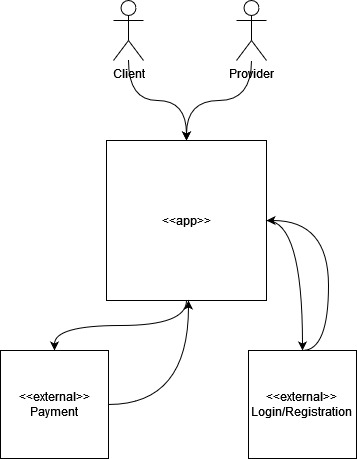
\includegraphics[width=0.5\textwidth]{assets/business_context.jpg}
    \caption{Diagram to describe the business context}
    \label{fig:business_context}
\end{figure}

\begin{table}[H]
    \setstretch{1.0}
    \begin{tabularx}{\textwidth}{lX}
    \toprule
    Artefact & Description   \\
    \midrule
    \gls{client} & Searches for a last time offer from a restaurant, bakery or pastry. \\
    \gls{provider} & Offers a still consumable product that was not sold during normal working time. \\
    Payment & Deals with the payment processing using registered information from another payment platforms. \\
    Login/Registration & Authenticated \glsplural{user} using logins from other platforms.  \\
    \bottomrule
    \end{tabularx}
\end{table}

A description of the existing elements will be described in our use case in table \ref{table_use_case}.
More elements of this view will be presented while discussing the internal decisions in chapter \ref{Patterns_Tacticts}. 

\newpage

\subsection{Structural view}

% put only big graphic and use it for on the 4+1 view

This following graphics are addressed to our technical team. They provide a deeper view of the model shown in
\ref{fig:business_context}. The once black-boxed elements showed above are now white-boxed so our development
team becomes a better understanding of the relevant components of the app.

\begin{figure}[H]
    \centering
    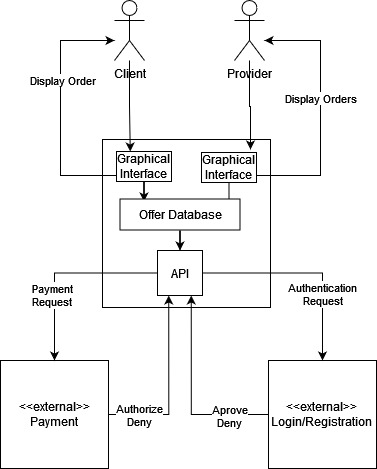
\includegraphics[width=0.4\textwidth]{assets/technical_context.jpg}
    \caption{Technical Context}
    \label{fig:technical_context}
\end{figure}

For the following graphic we choose a \gls{class diagram} to provide our development team a further view of the
structural elements of the project. This first class diagram gives a simple description of the classes that can
exist in the app.

\begin{figure}[H]
    \centering
    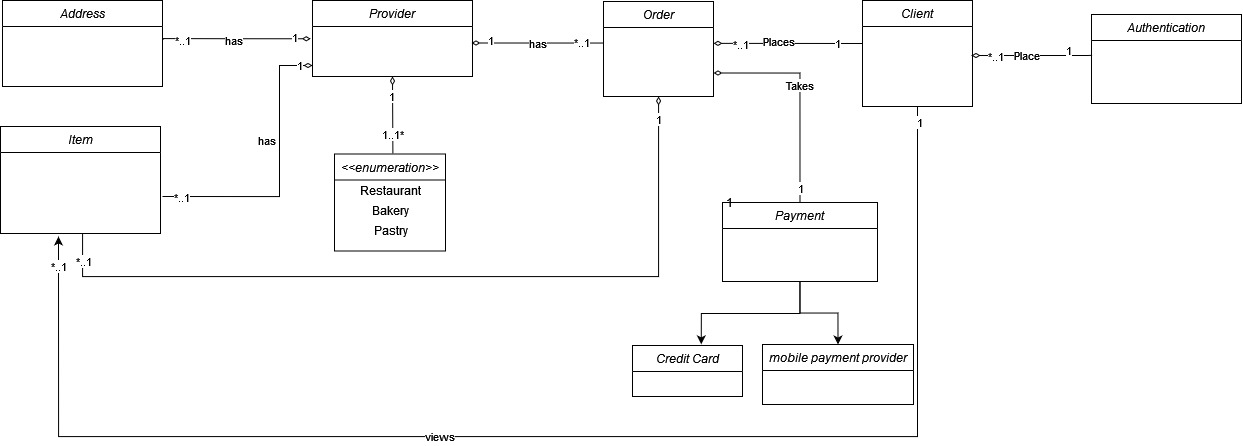
\includegraphics[width=1\textwidth]{assets/simple_classes_CD.jpg}
    \caption{Level 1 - Class Diagramm}
    \label{fig:simple_class_diagram}
\end{figure}

% The first part of the this diagram describes the element within the \gls{provider}. It contains one or more addresses and it 
% can offer one or more products. A provider will also fall into the category restaurant, bakery or pastry.

% \begin{figure}[H]
%     \centering
%     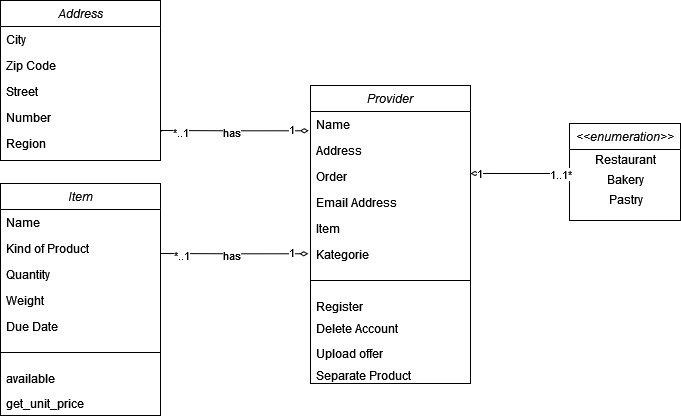
\includegraphics[width=0.6\textwidth]{assets/Provider_Addr_Item.jpg}
%     \caption{Provider overview}
%     \label{fig:Provider_addr_item}
% \end{figure}
 
% The class dedicated to the \glsplural{client} should be as simple as possible. It should provide basic interaction like
% registering, logging, deleting account, viewing product and placing order. The two last actions will stablish the communication 
% with the \glsplural{provider}.

% \begin{figure}[H]
%     \centering
%     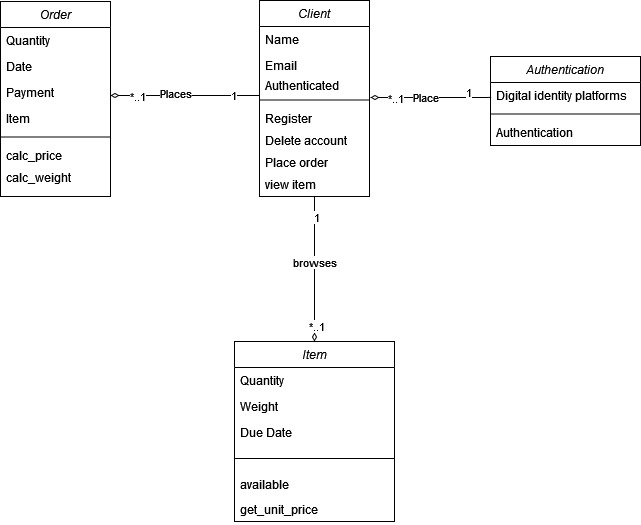
\includegraphics[width=0.6\textwidth]{assets/client_CD.jpg}
%     \caption{Client Overview}
%     \label{fig:client_CD}
% \end{figure}

% Finally we have an order placed by a \gls{client} and processed by a \gls{provider}. Here we will rely on a third party 
% to stablish the payment procedures.

% \begin{figure}[H]
%     \centering
%     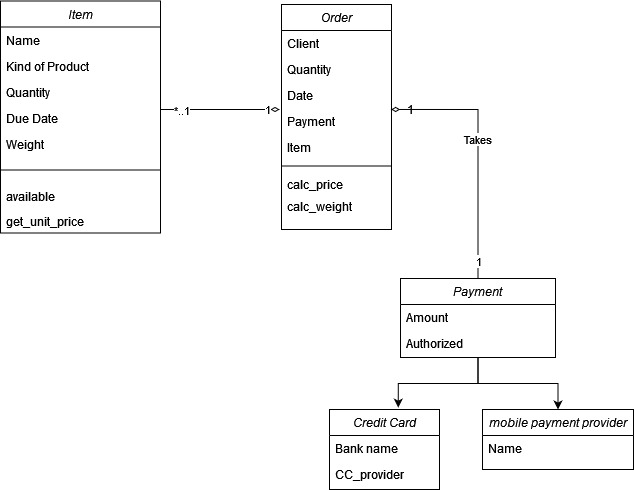
\includegraphics[width=0.6\textwidth]{assets/order_cd.jpg}
%     \caption{Order Overview}
%     \label{fig:order_cd}
% \end{figure}

\newpage
\thispagestyle{lscape}
\begin{landscape}

Zooming down the classes we presented before, we can see how they are build with its attributes, methods and
interaction with other elements.

\begin{figure}[H]
    \centering
    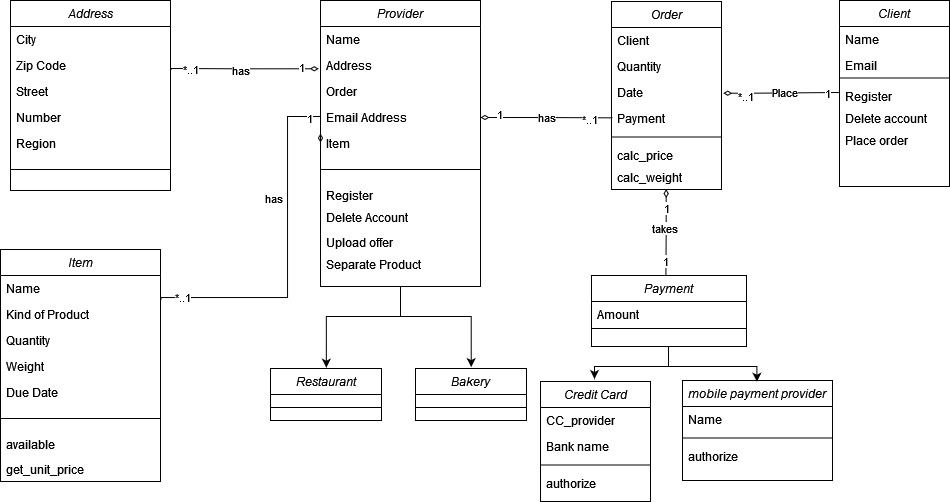
\includegraphics[width=1.5\textwidth]{assets/classes_CD.jpg}
    \caption{Classes Overview}
    \label{fig:class_CD}
\end{figure}

\end{landscape}

\subsection{Behavior view}

The following \gls{activity diagram} depicts the register and login procedure within the app. It should explain our
main stakeholders, \glsplural{provider} and \glsplural{client}, the starting process of the app.

\begin{figure}[H]
    \centering
    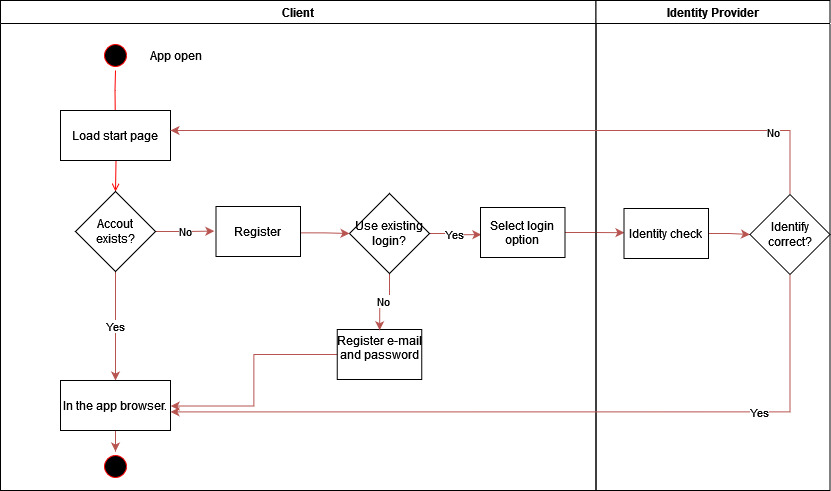
\includegraphics[width=1\textwidth]{assets/login_AC.jpg}
    \caption{Login procedures}
    \label{fig:login_register}
\end{figure}

To help understanding the above process we created the following \gls{sequence diagram} that depict the communication flow 
with the third party providers. 


\begin{figure}[H]
    \centering
    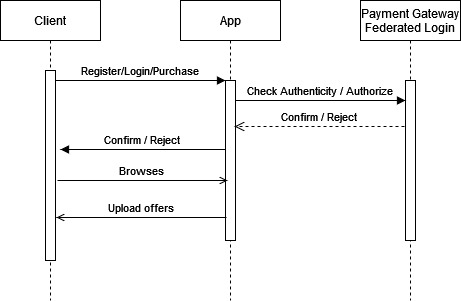
\includegraphics[width=0.7\textwidth]{assets/sequence_login_payment.jpg}
    \caption{Sequence of actions with third party applications}
    \label{fig:sequence_login_payment}
\end{figure}



